
\documentclass[final]{cmpreport}
\usepackage[]{algpseudocode}
\usepackage{placeins}
\makeatletter
\input{t1pcr.fd}
\makeatother
\setlength{\footnotesep}{3ex}
%%%%%%%%%%%%%%%%%%%%%%%%%%%%%%%%%%%%%%%%%%%%%%%%%%%%%%%%
%
%  Fill in the fields with:
%
%  your project title
%  your name
%  your registration number
%  your supervisor's name
%
%%%%%%%%%%%%%%%%%%%%%%%%%%%%%%%%%%%%%%%%%%%%%%%%%%%%%%%%
\title{Reversi Game Implementation}

%%%%%%%%%%%%%%%%%%%%%%%%%%%%%%%%%%%%%%%%%%%%%%%%%%%%%%%%
%
% The author's name is ignored if the following command 
% is not present in the document
%
% Before submitting a PDF of your final report to the 
% project database you may comment out the command
% if you are worried about lack of anonimity.
%
%%%%%%%%%%%%%%%%%%%%%%%%%%%%%%%%%%%%%%%%%%%%%%%%%%%%%%%%
\author{Kyle Alexander}


\registration{100082709}
\supervisor{Dr Christopher Greenman}
%%%%%%%%%%%%%%%%%%%%%%%%%%%%%%%%%%%%%%%%%%%%%%%%%%%%%%%%
%
% Fill in the field with your module code.
% this should be:
%
% for BIS            -> CMP-6012Y
% for BUSINESS STATS -> CMP-6028Y
% for other students -> CMP-6013Y
%
%%%%%%%%%%%%%%%%%%%%%%%%%%%%%%%%%%%%%%%%%%%%%%%%%%%%%%%%
\ccode{CMP-6013Y}

\summary{
Reversi is a 2 player board game where two players compete to gain the most pieces on the board when the game ends. Building a program that plays reversi involves storing the board and calculating whether players can make moves but this primarily the most complex part of the program is the compter opponent that will be used in the single player aspect of the program. 
In this report is an analysis of various algorithms used for both the search methods used in looking ahead in the game and the evaluation methods that can be used to judge a players position on the board programmatically. 

As part of the project the report was written for an implementation of Reversi has also been made and the report outlines the usages of algorithms in the program as well as a few tests and explanations as to why the implmentation did not perform well when compared to the theory that was implemented.
}

\acknowledgements{
I would like to thank Dr Christopher Greenman who provided advice throughout the year the this project was done and aslo due to his help on several data stractures and algorithms for the game that ended up in the final implementation of the program.
}

%%%%%%%%%%%%%%%%%%%%%%%%%%%%%%%%%%%%%%%%%%%%%%%%%%%%%%%%%%%%%%%%%%
%
% If you do not want a list of figures and a list of tables
% to appear after the table of content then uncomment this line 
%
% Note that the class file contains code to avoid
% producing an empty list section (e.g list of figures) if the 
% list is empty (i.e. no figure in document).
%
% The command also prevents inserting a list of figures or tables 
% anywhere else in the document
%
% Some supervisors think that a report should not contain these
% lists. Please ask your supervisor's opinion.
%
%%%%%%%%%%%%%%%%%%%%%%%%%%%%%%%%%%%%%%%%%%%%%%%%%%%%%%%%%%%%%%%%%%
%\nolist,

%%%%%%%%%%%%%%%%%%%%%%%%%%%%%%%%%%%%%%%%%%%%%%%%%%%%%%%%%%%%%%%%%%
%
% Comment out if you want your list of figures and list of
% tables on two or more pages, in particular if the lists do not fit 
% on a single page.
%
%%%%%%%%%%%%%%%%%%%%%%%%%%%%%%%%%%%%%%%%%%%%%%%%%%%%%%%%%%%%%%%%%%
\onePageLists
\begin{document}
\section{Motivation}
\section{Introduction}
The game of Reversi is a two player board game played on an eight by eight board using double sided circular pieces that are white on one side and black on the other. Of the two players one player is white and one is black and when the game is finished the player with the most pieces flipped to their colour wins. By tradition the black player moves first and the players take turns making moves by placing a piece with their own colour face up which then captures any pieces on the board that are between the placed piece and another piece of the players colour. A player can only play a piece in an empty square if the placement of the piece will capture at least one of the opponents pieces and if a player can not go the turn reverts back to the other player and when both players can not move the game is over.
\begin{cmpfigure}[htb]{Board before (Left) and after (Right) a move by white capturing pieces vertically up and diagonally up and left}
	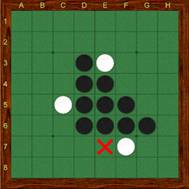
\includegraphics{othelloturn1.jpg}
	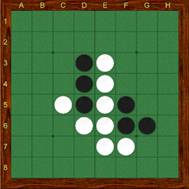
\includegraphics{othelloturn2.jpg}
\end{cmpfigure}
\FloatBarrier
Building an implementation of Reversi involves constructing a user interface for a human player to play the game through as well as storing the information about the board in data structures and keeping track of user input to place the users pieces and flip the colour of any pieces that the players move captures. Finally the program must have a computer opponent to allow single player and this is the most complex part of the program involving several elements of game theory such as decision trees and evaluation heuristics to build a computer opponent that can compete with a human player.

The report first consists of a brief history of computer Reversi detailing several milestones and also some significant existing pieces of software that have had major victories as computer opponents when playing against top level human players. 

Following this will be an analysis of existing algorithms used in the construction of a computer opponent. Some of these are used in the software built for the project and some not due to time constraints or they are alternatives that were not chosen.

After the analysis is the detailing of the implementation for the program that was built for the project. This will include explanations of the user interface and graphical aspects of the program, the underlying models used to store the board the game is played on and the decision algorithms implemented for the computer opponent.

Moving towards the end of the report the next chapter outlines the method used to determine the best weights for the evaluation function as several different algorithms are used to calculate a metric. These algorithms are combined to create a weighted mean that represents a players strength at that point in the game. The training method is used to calculate a good set of weights for the average.

A limited aspect of the project is the testing done between the computer opponent and other existing opponents that can be found online. The testing chapter will outline the tests performed and results that were gained.

Finally the last chapter contains a list of extra features that would be implemented given extra time and a plan on how the project would move forward with this time.
\section{History} 
Computer Reversi started as early as 1977 with Ed Wright creating a version written in Fortran that was published by Creative Computing \cite{Othello23:online} and later placed in the Games section of their \textit{Best of Creating Computing Volume 3} book that was published in 1980 \citet{TableofC3:online}

1 Year later Reversi would become a large part of Nintendo's history as they developed a digital tabletop arcade machine that played Othello that was the first game that Nintendo both published and developed.

With regards to the quality of Reversi Computer opponents A large milestone was made in 1980 with the first example of a machine outperforming a high level human player when the program Moor beat Hiroshi Inoue who at the time was the world champion at Othello.
From this point forward Computer Opponents in Othello only improved and in 1997 Logistello beat Takeshi Murakami who was also the world champion at the time but in this particular match Logistello won all six matches against the champion which solidified the idea that in the game of Othello computers had now surpassed the best human players.

In 1998 the creator of Logistello Michael Burro retired the program and as a result the development of computer Othello slowed but there are still examples that continue to be developed such as Saio and Edax. 
\section{Analysis of Existing Algorithms}\label{heu}
In a Reversi computer opponent and similarly in a Computer opponent for any two player game there are two base elements. These are the decision tree that is used to look ahead in the game and calculate moves based on the various possibilities several turns ahead and the evaluation function that is at least run at the terminal nodes of the decision tree to score the positional strength of a player for a given situation on the board.
\subsection{Minimax and Negamax}
Minimax and Negamax are both similar algorithms for constructing and traversing a decision tree. The initial decision tree is constructed by storing all the positions and colours of the pieces on the board and for each possible move of the player whose turn it would be simulating that move and constructing a child node in the tree containing the resultant board after performing the move and capturing the pieces. A decision tree will not be able to consider all possible moves for a single game as the amount of nodes that would need processing increases exponentially and depending on the speed of the algorithms for finding available turns and simulating those moves a decision tree may have a max depth of 3 to 16 \citet{SystemAr82:online} layers. 

Minimax is an abbreviation on minimum maximum and the concept behind the algorithm is the assumption that both players make the best possible moves when it is their turn. In a minimax tree each tree layer represents a players turn and moving down the tree the players alternate. Once the tree reaches its max depth the evaluation function is run on the terminal node and the value is stored in the node. Values are passed back up the tree depending on which player the parent node represents. As the tree will be used from the computer opponents perspective if the parent node is the same player as the computer opponent then the best possible move is taken from the child nodes and if the player of the parent node is the other player then the minimax algorithm takes the best move for that player which in turn is the worst move as far as our computer opponent is concerned\ref{minmaxpic}. Once the values are passed up to the root node of the tree the child node is chosen from the root node and the turn that results in this child node is the move used by the computer.
\begin{cmpfigure}[!htb]{Example of minimax passing values from terminal nodes to the root.\label{minmaxpic}}
	
	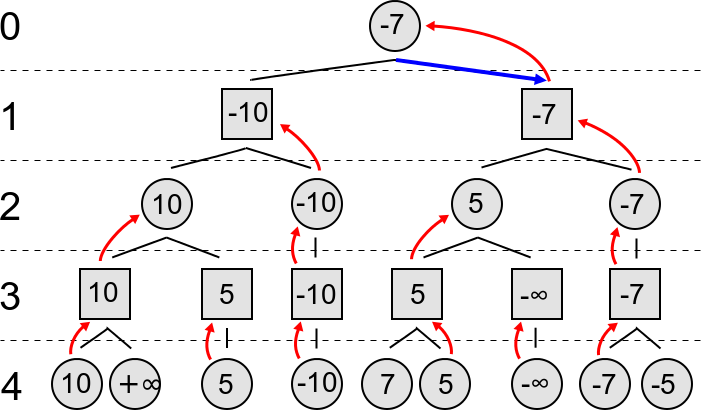
\includegraphics[scale=0.5]{Minimax.png}
	\\When the largest value is passed up the tree it is an example of the computer opponents move creating the children and when the smallest value is passed it is the players move creating the children
\end{cmpfigure}
\begin{cmpfigure}[htb]{minimax algorithm\label{minmaxalg}}
\begin{algorithmic}
\Function{minimax}{node, depth, maximizingPlayer}
\If{depth = 0 or node is a terminal node}
\Return the heuristic value of node
\EndIf
\If{maximizingPlayer}
\State $bestValue\gets-infinity$
\ForAll{children of node}
\State $v\gets$minimax(child, depth $-$ 1, FALSE)
\State $bestValue\gets$max(bestValue, v)
\EndFor
\space\Return bestValue
\Else
\State $bestValue\gets+infinity$
\ForAll{children of node}
\State $v\gets$minimax(child, depth $-$ 1, TRUE)
\State $bestValue\gets$min(bestValue, v)
\EndFor
\space\Return bestValue
\EndIf
\EndFunction
\end{algorithmic}
\end{cmpfigure}

\FloatBarrier
The negamax is a small alteration to the minimax algorithm that relies on the zero sum property of a two player game. Zero sum simply means that the gain of one player is equal to the loss of the other. Negamax utilises this fact to remove the if statement that checks to see if the player for the current node is the maximising player\ref{minmaxalg}. Due to the fact that Reversi is a zero sum game at any point in the decision tree finding the max of the children for the player who we are minimising (this is usually the human player) is equivalent to finding the minimum of our computer opponent who we are trying to maximise. In implementation this impacts the code in several ways. Firstly the above-mentioned if statement can be removed and only the block finding the max of the child heuristics needs to be implemented, secondly the recursive call to the algorithm must be negated to account for the alternation of players down the tree and finally the heuristic must be negated if the player at the terminal node is not our maximising player as the heuristic calculates positional strength for our maximising player. 

Of the two algorithms the minimax is implemented purely because the attempts at implementing negamax could not be made to work with the ability for start a new game with the computer going first or second. In the future remedying this conflict and implementing a negamax search would be done as even though only a single if statement is removed the algorithm is run many times every turn and so the time save would stack up making the change worth it.

\subsection{Quiscience Search and The Horizon Problem}
The Horizon problem is a problem inherent to the way decision tree and algorithms like the minimax algorithm look moves ahead in the game and it relates to the fact that the amount of nodes that need processing increases exponentially as said algorithm looks further and further ahead in the game. Normal Reversi at the current time is an example of an unsolved game and that means not all possible combinations of every move have been simulated to determine if there is a flawless set of moves. With regards to implementations of Reversi this means that an evaluation heuristic must be used to score the board. This is a hole in the computers ability to make a good decision as the computer opponent can be trapped by skilled players by a move being made to look favourable for the computer as far ahead as it can see but passed the computers ability to calculate moves ahead can be a move for the player that completely reverses the positions of each player leaving the player in a winning position.

The quiscience search is an addition to a search algorithm such as minimax that is used to attempt to solve the horizon problem by prioritising moves that an evaluation function has deemed interesting. During the project several heuristics for a quiscience search were implemented but none improved the computer opponents quality and given the extra time a quiscience can take the implementation was removed for the final program.

When the search finds an interesting node the sub tree for that node is prioritised and is usually run recursively to a depth larger than the predefined max depth of the tree to avoid traps. In Reversi an example of a heuristic that could be used would be to mark moves that play near the edges as interesting as it is possible to force a computer opponent that does not look far ahead to play a square that gives the player the corner or a semi stable edge piece.
\subsection{Tree Pruning}
Pruning the decision tree is crucial in being able to perform a search of a decision tree to a depth necessary for a competitive AI. The most common pruning is alpha beta pruning which stops the search running on a sub tree when a move is found to be worse than an existing move found earlier in the tree. With optimal move ordering alpha beta pruning can be used to prune the leaf nodes to $\sqrt{b^d}$ where b is the average number of children for each node on the tree and d is the depth of the tree \citet{ABmaths}.

Alpha beta pruning works by passing two extra variable up and down the tree that form a window. The two variable are alpha and beta with alpha being the lower bound of the window and beta being the upper bound. alpha and beta are changed to match the best heuristic found from child nodes and depending on whether the current node is trying to maximise or minimise the player alpha or beta get updated respectively. If alpha ever gets bigger than beta the window has effectively closed and the node is guaranteed to pass a value back up the tree that is worse than what has already been found.

\begin{cmpfigure}[htb]{A diagram demonstrating alpha beta pruning with cutoffs detailed}
	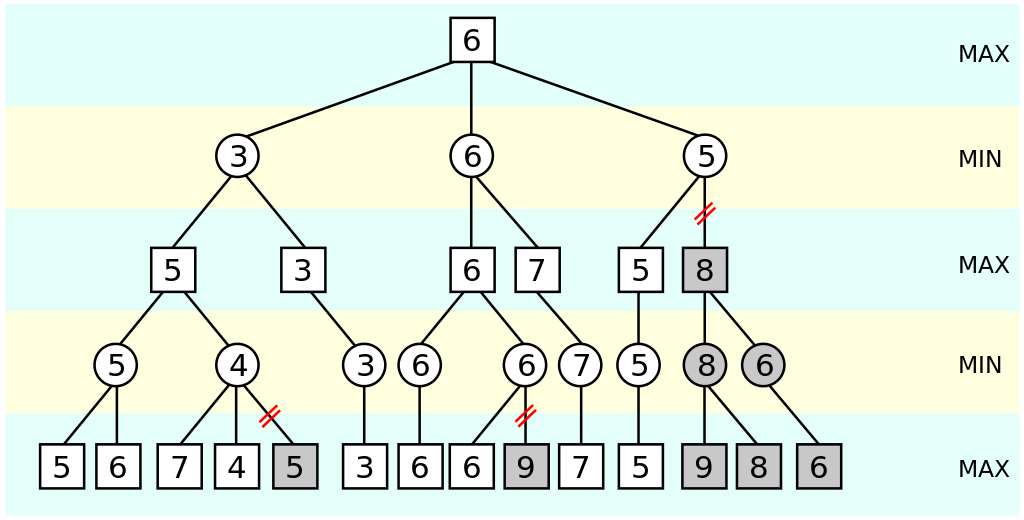
\includegraphics[scale=0.36]{AB.png}
\end{cmpfigure} 
\FloatBarrier
There are many pruning techniques that are extensions of alpha beta pruning. Killer heuristics is a method which keeps track of a pre determined number of moves per layer of the decision tree and the next time the search is run the stored moves are used to create children nodes first. The moves that are stored are moves that in previous searches generated the largest \textit{cutoffs} by the alpha beta pruning and the idea is that the moves will continue to create \textit{cutoffs} as the game progresses increasing the overall speed of the program as less nodes need to be processed.

If the search algorithm that is used is negamax instead of minimax then there is option of using negascout which is an algorithm similar to alpha bets pruning but uses the assumption of good move ordering when creating and processing child nodes. Negascout assumes that the first moves it checks when processing the children of a node is the best move or principal and it checks this by performing a search zero window alpha beta pruning which mean that alpha and beta are set to produce cutoffs regardless of results further down the tree. As the statement to decide if a cutoff occurs after the first recursive call to the first child the zero window search still covers all the nodes it assumes may be a principal variation. If there is value that return from the zero window search that is between the initial alpha and beta of the parent then the assumption about the first child is wrong and normal alpha beta pruning occurs.

With good move ordering negascout produces much more cutoffs than ordinary alpha beta pruning as it performs an initial search of the tree with a narrower window. The drawback of negascout id that if the move ordering is bad the initial zero window search will fail and the algorithm will effectively search the subtree twice costing time. Due to the fact that the software for the project uses minimax and not negamax negascout is not implemented.   
\subsection{Transposition Tables}
Transposition tables are used frequently in board game computer opponents as they can speed the search up for almost no cost. A transposition table is a table of existing board states that contain where all the pieces on the board are. This is useful as in Reversi it is possible to arrive at the same board state with several different combinations of moves and a transposition table can be used to quickly reference any results that came about when the same board state was previously processed. In particular the largest save computationally is the ability to conceptually merge the two nodes in the decision tree as from any given node in the tree the sub-tree from that node will always be generated the same. This is because no part of a decision tree node that is dependent on anything further up the tree than its direct parent. Due to this when two nodes have the same board state the sub tree for them will also be identical so only one needs to be processed.

Transposition tables can be implemented in the program for this project but have not been due to the lack of flexible data structures built into the C programming and time constraints have not allowed the necessary underlying data structures to be created as well as implementing the algorithm into the minimax search.
\subsection{Heuristics}\label{exheu}
The other essential part of the computer opponent besides the search algorithm is the evaluation function that takes a board state and returns the strength of a players position at that turn. There are several different methods that can be used to evaluate the board and while individually these algorithms provide poor results implementing several different heuristic algorithms and returning a weighted average provides the best result. Examples of heuristics include coin count, move count, weighting each position individually and finally piece stability. A table outlining the performance of the various heuristics can be found in section \ref{evalrefs} as the testable implementations of the algorithms is different to the explanations detailed below.


Coin count or coin parity is the simplest heuristic and consists of a simple count of each players pieces ad subtract the minimising players count away from the maximising players count. Coin parity is a very weak heuristic to base an computer player on as during early and mid game (0 to around 40 pieces on the board) having more pieces on the board correlates to having less available moves and given that a single move in Reversi can capture many pieces mobility is more important until later in the game.

As mentioned above mobility is an important part of early and mid game and so a heuristic that can be used is to measure the amount of moves available to each player given a specific board. A similar equation to the coin parity heuristic is used in that the number of moves available to the minimising player is subtracted from the the number available to the maximising player.

Another heuristic is counting the number of corners captured by each player as in Reversi corners hold a large strategic importance as once a players piece is placed on a corner it can not be captured. This heuristic can be used by itself similarly to the above heuristics or can be extended to assigning a value to each position on the board instead of just the corners. Depending on the strategic value of a position it is assigned a value. The values can be used by comparing them to a board and for each position if the maximising player has a piece on that square a counter is incremented by the value of the square and if the minimising player has a piece on that square the same counter is decremented. The result is a number that is higher if the maximising player has more pieces on strategically beneficial squares.

Finally piece stability is a measure of a pieces ability to be captured at some point in the future of a game. There are three levels of stability.
\begin{description}
	\item[Non-stable] A piece can be captured by the opponent on their next turn.
	\item[Semi-stable] A piece can not be captured the very next turn but can be captured at some point in the future.
	\item[Stable] A piece can not be captured for the rest of the game. An example would be a piece on a corner square.
\end{description}
By counting the amount of each players semi-stable and stable pieces and then subtracting the two as with the other heuristics the heuristic returns a higher value if the maximising has more stable/semi-stable pieces.
\section{Implementation}
This sections outlines the implementation of the program that was created as part of the project and also details how the algorithms in section \ref{heu} were used to create a computer opponent.

The program is written and compiled in C and uses an Object Orientated design. As c does not support classes the design is done by creating structs that contain what would be member fields of a class and functions that have at least  one argument which is a pointer to the struct as member functions. Each struct and its associated functions are implemented in a separate file to ease code readability. he exception to this is the Rect struct which is defined in the c file containing the entry point to the program as this struct is not used to in the modelling of the game but is used for window management and handling user input.
\subsection{Data structures and Algorithms}
There are several algorithms of note in the program that are not part of the AI and they are based around finding and making turns in the game. 

The underlying data structure for the board is two 64 bit unsigned integers that are initialised to zero and act as two bit masks containing the position of one colour of piece each. As they are 64 bits long they can be used to represent an 8 by 8 Reversi board and any set bits in the number represent the presence of a piece in that position. An example is the board that is used to start a game of Reversi.
\\
\\For the white pieces the bit mask is 68853694464
$$68853694464_{10} = 0000000000000000000000000001000000001000000000000000000000000000_2$$
which if we split into 8 rows of 8 looks like.
\\
\\
00000000\\
00000000\\
00000000\\
00010000\\
00001000\\
00000000\\
00000000\\
00000000\\
\\
And the 1s on this board denote where the white pieces would start at the beginning of the game. The same can be done with black pieces and the two numbers together hold all the information necessary for a Reversi board.

Two small algorithms using bit wise operations are used in the program to get and set individual pieces of a single bitmask as well as an algorithm used to flip pieces on both bit masks to perform a capture when given the colour of the capturing player and a third bit mask containing all the pieces that are captured.
\begin{cmpfigure}[htb]{Capturing pieces}
	\begin{algorithmic}
		\Function{flipCaptured}{\&whiteBitmask, \&blackBitmask, capturingBitmask, playerColor}
		\If{playerColor is white}
		\State $*whiteBitmask \gets *whiteBitmask | capturingBitmask$
		\State $*blackBitmask \gets *blackBitmask \& (\sim capturingBitmask)$
		\EndIf
		\If{playerColor is black}
		\State $*blackBitmask \gets *blackBitmask | capturingBitmask$
		\State $*whiteBitmask \gets *whiteBitmask \& (\sim capturingBitmask)$
		\EndIf
		\EndFunction
	\end{algorithmic}
\end{cmpfigure} 
\FloatBarrier

To find all the turns that can be made by a player the board searches iteratively over every square and for each square affectively spiders out in the 4 cardinal directions and the 4 diagonals. In each direction it performs the following algorithm
\begin{cmpfigure}[htb]{Algorithm for finding legal moves\label{legal}}
	\begin{enumerate}
		\item[1:] $availableDirection \gets FALSE$
		\item[2a:] If square is empty then End.
		\item[2b:] If Square is opponent then $availableDirection \gets TRUE$, move to next square in direction and goto Step 2. 
		\item[2c:] If Square is players piece and $availableDirection == TRUE$ goto step 3 otherwise End.
		\item[3:] Write all the positions iterated over in this direction to a bit mask
	\end{enumerate}
\end{cmpfigure}
\FloatBarrier

After the directions are iterated through any direction that reached step 3 has the resulting bit mask bit wise ORed with a final bitmask that represents all the pieces that placing a piece at the position captures.

\begin{cmpfigure}[htb]{Pieces vertically down and the downward left diagonal are both captured by the move highlighted in red}
	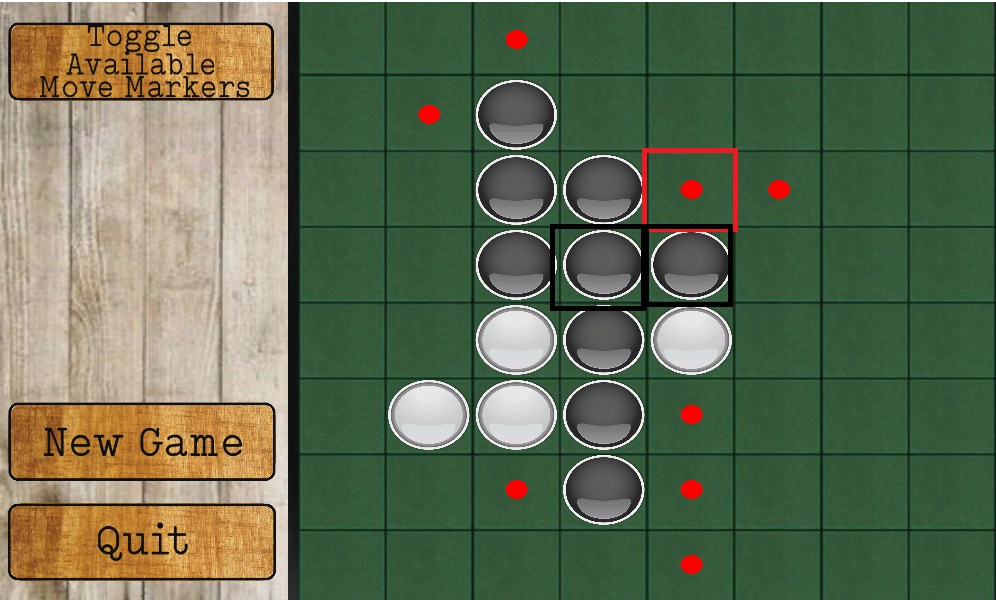
\includegraphics[scale=0.5]{capture.jpg}
\end{cmpfigure}  
\FloatBarrier

As well as the bit masks containing the locations of the data structure containing the board also contains a linked list which stores all the moves that can be made the player whose turn it is for that particular board. This is mainly used in the user interface to check if a clicked square is one of the available moves to the user but the storage of the available moves means the board can be passed through to the computer opponent without anything have to be recalculated.   
\subsection{Window Management and Rendering}
The program is written in C and uses Legacy Opengl for rendering. The library Freeglut is used to create and manage the window used for the program as well as handle user input. Due to the fact that OpenGL render with the origin at the bottom left and windows returns user mouse input from the board is user input is subtracted from the height of the window to align it with the drawing of the board. 

A rectangle struct is used to direct user input to the relevant buttons or the board and a contains function is used to determine if the user has clicked in any positions that need to respond to a click. Each button has a rect and the board has a rect and these are searched linearly to determine which response needs to be run. The user interface consists of a Reversi board and three buttons. The quit button exits the program, the new game button restarts a giving the user the option to go first or second and the Toggle move markers button enables or disables small red circles that highlight to the user which moves they can make.

A single render function renders the whole window and uses Opengl and the image loading library SOIL \citet{lonesock77:online} to draw textures that provide a nicer looking interface than block colour and shapes.
\subsection{Computer Opponent}
The implementation of the computer opponent in the software utilises many of the algorithms used in section \ref{heu} and the following subsections go into detail about the algorithms are implemented in the program.
\subsubsection{Minimax Algorithm}
The program uses a minimax search as the base for its search for finding the move it should make. A tree structure is used to store the tree as when recursing through the minimax search during a turn the most computationally expensive part of the search is using the available turns of the parent node to construct a board that is the same as the parent nodes board but with each turn applied to the board. Storing the tree between turns means that each level of the tree need to only be generated once which saves time overall as only the bottom two layers whenever the minimax search is performed. Storing the tree nodes also allows the added benefit of sorting a nodes children before recursing into any of them as the child nodes will not be generated as they are searched but already exist in the tree. Sorting the nodes will increase the performance of alpha beta pruning as mentioned in the next chapter. 
%TODO:expand ??
\subsubsection{Alpha-Beta Pruning}
The program implements alpha beta pruning and this is done by passing an alpha and beta value through to each recursive call of the tree search. The call to the root node of the tree search passes initial values of $-1000$ and 1000 respectively as it is impossible for the generated heuristic to be outside these values. During the search alpha and beta are changed based on the result of the recursive calls to the tree. Alpha is changed if the node is for the maximising player and the heuristic is larger than our current alpha, similarly beta is modified if the node is for the minimising player and the heuristic is smaller than our current beta. Together this results in alpha and beta forming a window that becomes more narrow as better variations are found and finally alpha becomes larger than beta, the window closes and a cutoff occurs.
\subsubsection{Evaluation Functions}\label{evalrefs}
The Program uses a weighted average of piece stability, a static board scoring individual positions and finally a mixture coin parity and movement count. During late game the program uses a coin count as mobility is limited during late game regardless of the employed strategy and unless at some point the program tries to maximise coins then it will never be trying to win. Before the late game the same weight for the coin count is used in the algorithm to maximise the number of available moves.

Given that in the program counting semi stable and counting completely stable pieces are weighted differently there are four individual algorithms that can be compared and to test the performance of each individually computer vs computer runs of Reversi games are run and the results are listed below. Given that there is no randomness in the heuristic algorithms only two tests need to be performed between each heuristic, one each for each heuristic going first.


\begin{cmptable}[htb]{Comparison of each individual heuristic algorithm}
	\begin{tabular}{|p{3cm}|p{3cm}|p{3cm}|p{3cm}|p{3cm}|}
		\hline
		 Going first to the right and going second down & Piece and move count & Static board values & Semi stable piece count & Completely stable piece count \\ \hline
		Piece and move count & Na & Piece count wins & Piece Count wins & Piece Count wins\\ \hline 
		Static board values & Static Board wins & Na & Static Board wins & Static Board wins\\ \hline 
		Semi stable piece count & Stable piece count wins & Stable piece count wins & Na & Semi Stable piece count wins \\ \hline 
		Completely stable piece count & Stable piece count wins & Stable piece count wins & Completely stable piece count wins & Na\\ \hline 
		
	\end{tabular}
\end{cmptable}
\FloatBarrier
The table demonstrates that either all the heuristics perform equally and the advantage goes to which computer plays second or the computers decision tree is broken in a way that has not been found and plays worse when going first.

piece count and move count are simple algorithms with piece count being a hamming weight of each bitmask and the move count employs the same algorithm as in figure \ref{legal}. The use of the the static board is outlined in section \ref{exheu}. The following board is used in the program for evaluating positions.

\begin{cmptable}[htb]{Static positional strength board}
	\begin{tabular}{c|c|c|c|c|c|c|c}
		500 & -25 & 20 & 10 & 10 & 20 & -25 & 500 \\ \hline
		-25 & -25 & 1 & -5 & -5 & 1 & -25 & -25 \\ \hline
		20 & 1 & 5 & 2 & 2 & 5 & 1 & 20 \\ \hline
		10 & -5 & 2 & 1 & 1 & 2 & -5 & 10 \\ \hline
		10 & -5 & 2 & 1 & 1 & 2 & -5 & 10 \\ \hline
		20 & 1 & 5 & 2 & 2 & 5 & 1 & 20 \\ \hline
		-25 & -25 & 1 & -5 & -5 & 1 & -25 & -25 \\ \hline
		500 & -25 & 20 & 10 & 10 & 20 & -25 & 500 \\
	\end{tabular}
\end{cmptable}
\FloatBarrier
From the table it is evident to see the importance placed on acquiring corners but also penalises the adjacent squares as having a piece in these squares will normally give a skilled player the corner. Apart from this there is an increase on value for the edges and a similar but less harsh penalisation for moving on squares that can give the edges away.

Calculating piece stability is more complex and while whether a piece is semi stable is easy to calculate as a check to see if one of the opponents available moves captures the piece can be done whether a piece is completely stable is more difficult. In Reversi a piece is completely stable if it can not be captured and this means that of the eight surrounding squares there are at least four adjacent squares that either contain a stable piece themselves or the square is off the board. In the game this means corners can be used as initial stable squares as a corner square has five adjacent squares that are off the board. In implementation the program does this using an algorithm that first checks to see if there are four adjacent pieces that are off the board or stable and then tests to see whether there are adjacent pieces from the ones found. As the algorithm relies on other pieces being already deemed as stable the algorithm works from the corners inwards to the centre of the board when iterating through the squares on the board. This algorithm is only an estimate as there are special cases where pieces can become stable as they are in completed rows, columns and diagonals.
\section{Training}
Given that a good heuristic is paramount to having an opponent that can compete with human players choosing the weights for each of the methods in section \ref{evalrefs} correctly is a very important part of the program.

To find appropriate weights he program can be compiled in an alternative training mode the plays various configurations of the computer opponent against each other to find the one that provides the most wins. The training uses a winner stays on approach and creates opponents with different weights for the heuristics and keeps who wins from the previous winner and the newly generated opponent. If a computer wins more than 5 times against consecutive generated opponents the weights used to generate that computer are written to a log file that can be used to compile the normal program with the best found heuristics.

\begin{cmptable}[htb]{Number of wins for weights that won more than 3 games in a row when training \label{weights}}
	\begin{tabular}{|p{2cm}|p{2cm}|p{2cm}|p{2cm}|p{4cm}|}
		\hline
		Static board weight & piece and move count weight & Complete stable count & Semi stable count & wins \\ \hline
		22 & 14 & 90 & 71 & 4 \\ \hline
		22 & 53 & 35 & 79 & 9 \\ \hline
		28 & 83 & 37 & 66 & 4 \\ \hline
		25 & 13 & 21 & 63 & 5 \\ \hline
		19 & 54 & 15 & 27 & 5 \\ \hline
		31 & 36 & 25 & 38 & 4 \\ \hline
		36 & 78 & 13 & 69 & 4 \\ \hline
		3 & 53 & 93 & 72 & 4 \\ \hline
	\end{tabular}
\end{cmptable}
\FloatBarrier

These weights were found by performing 1000 games of the computer playing against itself and of all the successful sets of weights the second row in the table was by far the most successful set of weights. For the testing in section \ref{tests} the weights from that row will be used.
\section{Results Versus Other Computer Opponents}
Due to a lack of automated test environment there is a limited number of tests. Moves were hand made between clients and in total the program was tested against 10 other opponents. There is no randomness in the projects program so depending on whether the client our program is being tested against has randomness sometimes only one test needs to be performed and other times multiple tests need to be done and averaged. 

\begin{cmptable}[htb]{Tests performed between the project implementation and various other implementations of Reversi/Othello}
	\begin{tabular}{|p{4cm}|p{4cm}|p{4cm}|}
		\hline
		Test Opponent & \multicolumn{2}{|c|}{Project Implementation}\\ \hline
		& Project going first & Project going second \\ \hline
		\url{www.coolmath-games.com/0-reversi} at medium difficulty & Test opponent won 6 to 4 & Test Opponent does not support going first \\ \hline
		\url{www.coolmath-games.com/0-reversi} at easy difficulty & Test opponent lost 8 to 2 & Test Opponent does not support going first \\ \hline
		\url{www.web-games-online.com/reversi} & Test Opponent won 10 to 0 & Test Opponent won 10 to 0 \\ \hline
		\url{www.gamesforthebrain.com/game.reversi} & Test opponent won 7-3  & Test opponent does not support going first \\ \hline
		\url{www.neok12.com/games/reversi/reversi.htm} & Test opponent drew 5-5  & Test opponent does not support going first \\ \hline
	\end{tabular}
\end{cmptable}

As seen in the table the implementation does not perform well and its only victory is against an easy opponent which during the game did not take corners and strategically important squares when given the opportunity to do so. During all tests the program consistently gave away corner squares to the opponent and as there is no randomness the moves c3, b2 and a1 always resulted in a player going second against the program getting a corner. This is contradictory to the heuristics as the static board values values corners very high which means the program should aim to take squares and only give them away as a last resort. This could be the result of a bug in the minimax search or the result of the other heuristic methods.
\section{Further Development}
In the future the priority would be to develop the minimax tree into a negamax tree that uses negascout on top of the existing alpha beta algorithms. Using good move ordering this would increase the speed of the search allowing for deeper searches hence improving the ability of the computer opponent as it would be able to avoid traps that could be made outside of the existing computers ability.

Due to the results of the testing it is clear that a better heuristic function is needed and after the search has been sped up this would be the next thing to fix. Before any other features are added the AI should at least be able to compete and win against other Reversi implementation that can be found on browser games websites. Once a more competitive heuristic is made te possibility of adding difficulties to the program can be considered.

Part of the improvement of the heuristic would involve a more sensible training method that instead of randomly choosing opponents for the previous winner to pay against the next opponent could use weights from the previous winner but adjusted slightly and slowly trends could be found for various weights with ideal values eventually being found.
\section{Glossary of Terms}
Below is a table outlining several terms used throughout the report that may be unclear and the relevant explanations of those terms.
\begin{cmptable}[h]{List of terms \label{glossary}}
	\begin{tabular}{|l|p{10cm}|}
		\hline
		Computer Opponent & An AI Reversi Player \\ \hline
		Move ordering & When creating children a node will process the list of possible moves and create a child for each. If the tree is maintained between turns the moves can be ordered based on the heuristic value of a node even if it not a leaf. \\ \hline
		Cutoff & If alpha is ever bigger than beta in alpha beta pruning then a node will stop looping through its children and the rest of the subtree is left unprocessed. This collection of unprocessed nodes form the cutoff \\ \hline
		Board state & information containing the location and colour of all the pieces on the board \\ \hline
		Variation & A variation is a line that goes from the root node of a decision to a terminal node and represents a single sequence of moves made from the current board.\\ \hline 
		Hamming Weight & An algorithm that counts the number of bits set in a bitfield see \cite{wiki:hamming}.
		\\ \hline
	\end{tabular}
\end{cmptable}
\clearpage
\bibliography{final.bib}	
\end{document}